\documentclass{article}
\usepackage[margin=1.2in]{geometry}
\usepackage[colorlinks=true, allcolors=blue]{hyperref}
\usepackage{graphicx}
\usepackage{float}
% \usepackage[capitalise]{cleveref}
\usepackage{ctex}

\begin{document}
\title{算法笔记}
\author{麦业民}
\date{}
\maketitle
\setlength{\parindent}{0em}

\section{简介}
\label{sec:intro}
这是本人刷\href{https://leetcode.cn/}{LeetCode}所留笔记。其中涵盖了各种算法设计思想:
\begin{itemize}
    \item 动态规划
    \item 双指针
    \item 二分法
\end{itemize}
以及各种数据结构:
\begin{itemize}
    \item 数组(字符串)
    \item 散列表
    \item 栈
\end{itemize}
\par
算法皆以Python3实现。简单题只做简略描述。

\section{题目}
\label{sec:questions}

\subsection{三数之和}
\label{sec:three-sum}
此题官方难度为中等,实际中等偏难,通过率为$38.65\%$,运用了双指针、散列表。

\subsubsection*{问题描述}
% 给你一个整数数组$a_n$,判断是否存在三元组$(a_i,a_j,a_k)$满足$i\ne j\land i\ne k\land j\ne k$,同时还满足$a_i+a_j+a_k=0$ 。请你返回所有和为 0 且不重复的三元组。
% \par
% 注意:答案中不可以包含重复的三元组。

\begin{figure}[H]
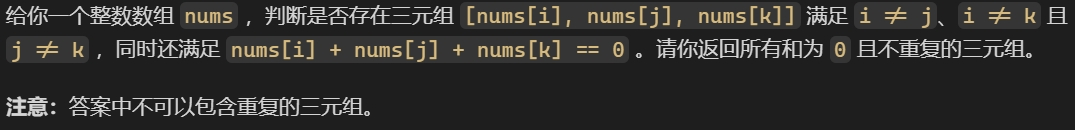
\includegraphics[width=\linewidth]{img/15-1.png}
\end{figure}

\subsubsection*{示例}
\begin{figure}[H]
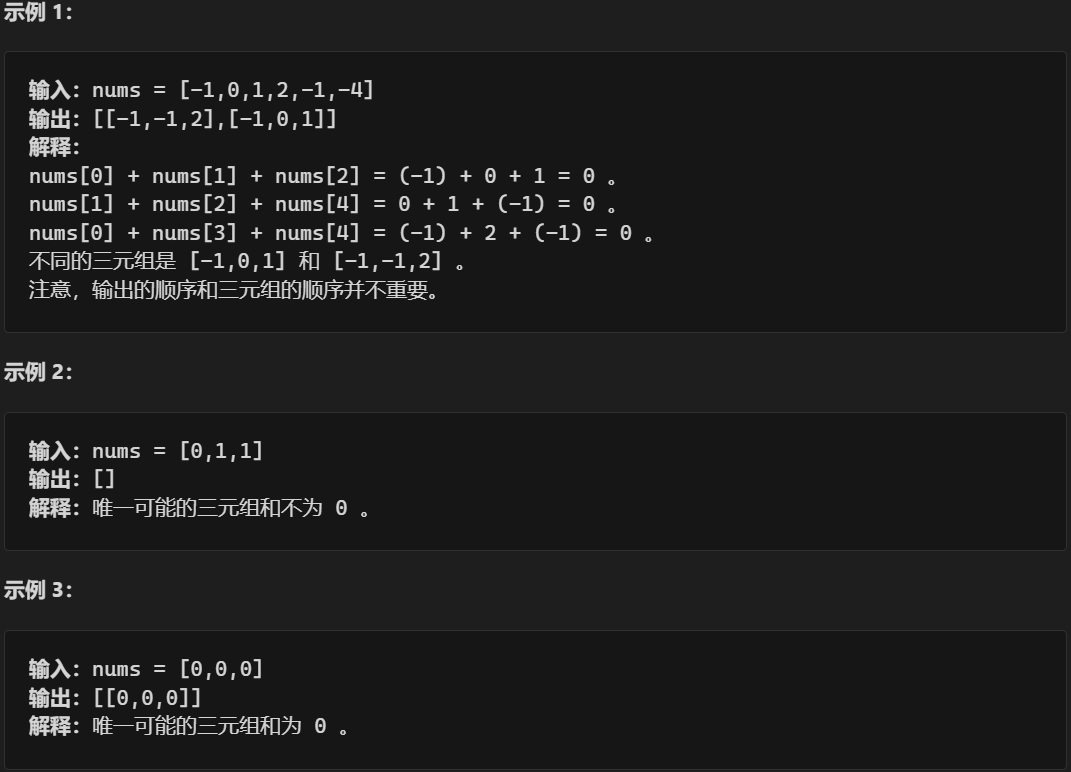
\includegraphics[width=0.8\linewidth]{img/15-0.png}
\end{figure}

\subsubsection*{思路}
固定其中一个数,将其转换为两数之和问题(参见\ref{sec:two-sum})。由于两数之和问题要求输入有序且只有唯一解,所以我们需要对上述输入进行排序,并再找到

\subsection{两数之和}
\label{sec:two-sum}
abc

\end{document}